\Chapter{Megvalósítás}

%Ez a fejezet mutatja be a megvalósítás lépéseit.
%Itt lehet az esetlegesen előforduló technikai nehézségeket említeni.
%Be lehet már mutatni a program elkészült részeit.
%Meg lehet mutatni az elkészített programkód érdekesebb részeit.
%(Az érdekesebb részek bemutatására kellene szorítkozni.
%Többségében a szöveges leírásnak kellene benne lennie.
%Abból lehet kiindulni, hogy a forráskód a dolgozathoz elérhető, azt nem kell magába a %dolgozatba bemásolni, elegendő csak behivatkozni.)
%A stílusfájlok a \texttt{styles} jegyzékben találhatók.
%A stílusok között szerepel még C++, Java és Rust stílusfájl.
%Ezek használatához a \texttt{dolgozat.tex} fájl elején \texttt{usepackage} paranccsal hozzá kell adni a stílust, majd a stílusfájl nevével megegyező környezetet lehet használni.
%További példaként C++ forráskód esetében ez így szerepel.
%\begin{cpp}
%#include <iostream>
%
%class Sample : public Object
%{
%    // An empty class definition
%}
%\end{cpp}
%Stílusfájlokból elegendő csak annyit meghagyni, amennyire a dolgozatban szükség van.
%Más, C szintaktikájú nyelvekhez (mint például a JavaScript és C\#) a Java vagy C++ %stílusfájlok átszerkesztésére van szükség.
%(Elegendő lehet csak a fájlnevet átírni, és a fájlban a környezet nevét.)
%Nyers adatok, parancssori kimenetek megjelenítéséhez a  környezetet lehet használni.
%\begin{verbatim}
%$ some commands with arguments
%1 2 3 4 5
%$ _
%\end{verbatim}
\Section{Kezdetek}
Még a téma megfogalmazása előtt eldöntöttem, hogy a szakdolgozatomhoz tartozó programot C\# nyelven fogom írni. Ennek legfőbb oka az eddig megszerzett nyelvi jártasságom. Magát a nyelvi verziót és a program alatt futó keretrendszert viszont a feladathoz igazítottam. Először a .NET Core 5 lett kiválaszva de kényelmi okokból, illetve mivel a platformfüggetlenség nem volt elsődleges szempont ezért  a .NET 4.7.2-es verziója lett a projekt keretrendszere. Egy érdekes tapasztalat, hogy a NuGet pkg-ket legtöbbször nem sikerül a fejlesztőknek egy éven belül frissíteni, ezért sokszor nem célszerű az éppen legfrisseb .NET verziót használni. (A kívánt pkg-k frissülése után a projekt is .NET 4.8-ra lett migrálva.) A NuGet a C\# csomagkezelője. Már megírt modulok találhatóak rajta, melyek között van ingyenes és licenszelhető is. A C\# alatt elérhető leggyakrabban használt fő alkalmazástípusok, a(z):
\begin{itemize}
\item ASP Web projekt és a hozzá választható FrontEnd\\
\item Windows Console alkalmazás (Főként utility projektekhez használják)
\item Windows Forms "klasszikus" ablakos alkalmazás gombokkal és textboxokkal. (Leginkább a kétezres évek formavilága)
\item WPF (Windows Presentation Forms) Az előző egy "felújított" változata. Ez lényegesen több opciót biztosít a felhasználói felület testreszabására.
\end{itemize}

A projektválasztás a Windows Forms alkalmazástípúsra esett. (továbbiakban WF) A WF ugyan csak egyszerű grafikai megjelenítést tesz lehetővé, de egy gráf, vagy háló folyamatai könnyedén megjeleníthetőek. A WF cserébe könnyebben szerkeszthető mint egy WPF XAML nyelven leírt felülete, és kevesebb erőforrást is igényel. 
\newpage
\Section{Felépítés}
A fentebb említett verziókülönbségek miatt a projektet csak 4.7.2-es .NET alatt lehetett létrehozni. A projekt eredetileg egy TDK-hoz készült, később viszont módosítva lett. Az alkalmazás felépítése a következő: 

\begin{figure}[h!]
\centering
\includegraphics[scale=0.6]{images/scheme.png}
\caption{Az alkalmazás vázlatos felépítése}
\label{fig:scheme}
\end{figure}

\textbf{FileManager / Parser } Feladata az XML file beolvasása, és tagolása. Az így feldolgozott adat kerül átalakításra a program későbbi szakaszában.\\
\textbf{Converter} A program fő része. Feladata a már tagolt adathalmaz átalakítása. Az átalakított adathalmaz DLV formátumba kerül, majd gráfleíró nyelvre. (DOT) Az így előállított háló menthető egy fileba.\\
\textbf{Display} Megjelenítő modul a konvertált háló UI-ra rajzolásáért felelős. Kis háló esetén az animáció is lehetséges.\\
\textbf{Analyzer} A hálón végezhető elemzéseket végzi el. Majd ezek eredményét megjeleníti, illetve elmenti. 

\Section{FileManager / Parser }
A File manager a C\# hagyományos XML megoldásait használja, ez az \textbf{XmlDocument} és \textbf{XmlReader} osztály illetve a hozzá tartozó metódusok. A felhasználói felületen a felhasználó által kiválsztott file kerül a managerbe. A C\# támogatja az XML fileok hagyományos XPath alapú feldolgozását, azonban elérhető egy gyorsabb XML feldolgozás LINQ-val. A LINQ a C\# nyelvbe integrált query nyelv. Szintaktikája az SQL éhez hasonló annyi különbséggel, hogy a 'SELECT' a query végére kerül az eleje helyett. Ez főként a kódban előforduló lekérdezések elkülönülése miatt lett így tervezve. 
\Section{Converter}
A Converter a program fő modulja. A leképzés fejezetben felsorolt nyelvi elemeket dolgozza fel és készíti el a részhálókat, amiket aztán összefűz. Konverzió során az XML soronként kerül feldolgozásra. Egy átolvasás után a nem szorosan illeszkedő részek, mint részhálók, segéd folyamatok stb. külön szálok kerülnek feldolgozásra aszinkron módon. Ezzel a konverziós idő (a modelltől függően) rövidül. A konverzió gyakorlatilag egy keresés egy Dictionaryben. A Dictionary egy kulcsot vár ami alapján egy értéket ad vissza. (Pont, mint egy valós szótár, ahol a kulcs az idegen nyelvű szó, az érték pedig a szó magyar megfelelője). Egy kisebb méretű Dictionary keresés durván $O(n)$ , ha $n$ darab elemre keresünk, ugyanis a \texttt{Dictionary.Contains()} egy elemre $O(1)$ komplexitású. Keresés után ezeket még rendezni kell és összefűzni. Ez utóbbi szintén minden elemre végbemegy, de ve egyidejűleg egy validáció is. A konverzió során az XML elem attribútumai és gyerekei alapján kerül az elem a háló egy adott pontjára. Ez egy újabb $O(n)$ lépés. Ha a rész szálak kész vannak és a fő szál is elkészült a részek egy hálóba lesznek rendezve ami $O(s)$, ahol az $s$ a részhálók száma. Idáig a program tehát $O(2n+s)$ lépést tesz meg. 
\Section{Analyzer}
Az analyzer feladata az ötödik %MAKE IT REF!!!!!
 fejezetben leírtak gyakorlati alkalmazása az elkészült hálóra. Az analyzer eredetileg pythonban lett megírva. Ezt az indonkolta, hogy az akkori alapalkalmazáshoz külön készült, mintegy kiegészítőként. Később a programba integrálva lett. Előszor IronPython alatt került bele, később teljesen átírva AGLIB-hez, majd mégegyszer átírva jelenlegi Google OR toolset leírónyelvre. Az IronPython a python nyelv .NET-en futó implementációja. Gyakorlatilag kicsit gyorsabb a hagyományos pythonnál de cserébe a platform-függetlenséget feláldozza. (Jelenleg viszont az új .NET verzió futtatható Linux és MacOS rendszeren is.) Az AGLIB egy analitikus csomag aminek csökkentett képességű verziója elérhető a NuGet rendszerén keresztül ingyen. (A teljes verzió viszont licenszköteles.) A jelenleg használt Google OR tools egy ingyenesen elérhető open source software csomag optimalizáláshoz,LP, CP programozáshoz, illetve útválasztásos és flow feladatok megoldásához. A csomag előnye a felépítésében rejlik. A probléma leírása után egy proto állomány  készül, amit egy solver fog megoldani. A solver LP problémáknál a GLOP, de külső solver is használható. A solverek implementáltak több platformra is. Az elérhetőség és a független problémaleírás eredménye, hogy az OR tools támogatott C++, C\# , JAVA és Python nyelven is.
 
\Section{Kezdeti nehézségek}
Miután körvanalazódott a feladat megvalósításának menete, létre hoztam egy kanban táblát a fejlesztési folyamatok nyomonkövetéséhez. (Ez a verziókezelővel együtt online, az Azure felületén érhető el.) A táblában különböző lebontásokban látható, a fő és rész egységek, valamint a feature-ök és tesztek. Az első lépés a BPEL nyelv megismerése volt. A BPEL-hez található anyagok nagy része hagyaték anyag, ugyanis a BPEL alapú folyamatkövetés kiszorult a népszerűségből. Ennek több velejárója van, de a leg szembetűnőbb, az aktívan elérhető segítség hiánya, a már hiányos dokumentáció, vagy éppen a dokumentációban felsorolt anyagok elérhetőségének hiánya. A program készítése során kellett generálni egy úgymond tanító anyagot, amely a program részeit érthetően elmagyarázza, és későbbiekben lehet használni a konverzió és a feldolgozás helyességének ellenőrzésére. Ezen tesztadatok legenerálása sokkal nagyobb nehézséget jelentett, mint vártam, vagy mint a program többi részének egy hiba utáni javítása. \\
Ismerjük meg a generáláshoz szükséges feltételeket! A BPEL írására lehet egy sima szövegszerkesztőt alkalmazni, de ez nem célravezető, mivel a háttér XML validációja kézzel nehézkesen oldható meg. A leggyakrabban hivatkozott szerkesztő az ECLIPSE. Az IDE nem támogatja alapértelmezetten a BPEL szerkesztését, ezért egy beépülő szükséges. A rendszer egy url megadása ellenében az adott szerveren tárolt beépülők letöltését, regisztrációját és integrálását teszi lehetővé. A folyamat több helyen is félre tud siklani, először az Eclipse verziójának különbözetében, aztán a szerver által alkalmazott biztonsági beállításokon, legutoljára az operációs rendszer jogosultságkezelésén. Sajnos a legfrisebb verziójú Eclipse nem támogatja a már idejét múlt szerkesztőt, ezért v6.0 körüli IDE-t kell telepíteni. A telepítés sajnos csak hagyaték rendszeren végezhető el. (ez lehet mind Linux, mind Windows). A programnak Windows 2000/Xp a rendszerkövetelménye hisz egy durván 2000-2002 es rendszerről beszélhetünk. Szerencsére a hagyaték rendszerek terén előzőleg szerzett tapasztalataim segítségemre voltak. A kettő Windows dual-boot egy korhű gépre telepítése után az editor hajlandó volt települni, egy azt megelőző gyakorlatilag verzióhekkelést követően. A frisebb Eclipse-el el kellett hitetni, hogy az állomány friss, de nem szabad volt feltelepítettni, hanem az így kinyert köteget kellett a másik gépen az Elcipse alá telepíteni manulisan. Az IDE beállításai után lehetőség nyílt egy program szerekesztésére, de ekkor még csak validálatlan formában. Ekkor kiderült, hogy a szekresztés befelyézéhez és validáiójához egy szerverre van szükség. A szerver lehet local szerver is. A jelenleg Oracle kézben levő rendszer ehhet nem ad segítséget, de interneten található hozzá segédanyag.\cite{helloworld} Az ebből megismert Apache és ODE szerver szintén csak korhű rendszeren tud futni. A helyzetet bonyolítja, hogy a Ode-War állományokhoz jre + jvm is szükséges. A jre egy bizonyos verziója viszont inkompatibilis az ode war állomány kifejezetten ahhoz tervezett verziójával. A jre, apache tomcat, ode verziók közösen nagyon kevés működő kombinációt engednek meg. Ennek ellenére, a telepítés befejeztével a legenerált minta még mindig nem ellenőrizhető, hiszen a szervernek futnia is kell. Ellenben a futó szerverbe fel kell regisztrálni az Oracle validációs szerverét, ahonnan egy aktuális sémát vár. A letöltött séma gyakorlatilag  a BPEL verziót határozza meg. Sajnos ez a szerver 2010 óta nem működik, így a hosszadalmas munka után nem várt végeredményhez jutottam. Az így felállított rendszerrel 10 darab BPEL állományt generáltam, de mivel nagy része szerveresen állítható és kapcsolat nélkül helyfoglaló szöveg van kulcsfontosságú helyeken, így a minta felét el kellett dobni, mert szemmel láthatólag nem volt helyes. A mintagenerálást két hónap elteltével később újra megpróbáltam egy virtuális gépen ezúttal, de ekkor még kevesebb eredmény született, ugyanis az Oracle ekkor kezdte a repository-k újraszervezését. Az egy hetes átszervezés után tapasztaltam, hogy a projektet nyugdíjazták, és jelnleg sem érhető el csak a hagyaték oldalon, de tényleges letölthető forrás nélkül. A dolgozat ezen fejezetének írásakor az oldal még mindig nem elérhető. 

\Section{A converter }
A konverzió kezelését különösen problémásnak gondoltam. Tanulmányaim során sose volt említve összetettebb adattípusok feldolgozása és azok közötti konverzió. Először egy kétszeresen összetett adattípusban gondolkoztam ami gyakorlatilag egy véges, két dimenziós tömb, hiszen a BPEL csak véges számú elemet tartalmaz gyárilag, és a szabadon definiált elemekkel nem foglalkozunk. A tömb egyik dimenziója a bejővö BPEL elem, a másik pedig a hozzá tartozó előre meghatározott konverzió eredménye. Később eszembe juttott a szakmai gyakorlat alatt szerzett információ a C\# ban natívan jelen levő összetett adatstruktúráiról. Így esett a választás végül a Dictionary-re. A Dictionary egy 'Key - Value' azaz kulcs és érték alapon működő tár. Használata során egy kulcssort kell gyártani a rekordok számára, és a kulcshoz tartozó értéket felvinni. A Dictionary runtime, azaz futás idő alatt bővíthető ha szükséges, de mivel csak előre definiált elemeket használunk, ezért ez kihasználatlan marad. Konverzió során külön kell kezelni a színes és egyszerű Petri-hálót. Az egyszerű hálós konverzió során sokat segített Christian Stahl által közzétett publikáció\cite{bpelToPnet}.

\Section{Vizualizáció}
A vizualizáció az alábbi módon történik:
\begin{figure}[h!]
\centering
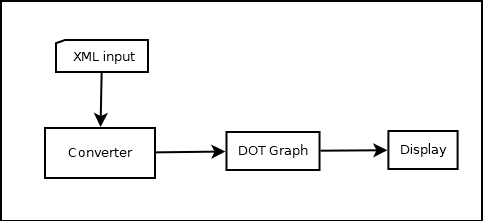
\includegraphics[scale=0.6]{images/graphdisplay.png}
\caption{A vizualizáció menete}
\label{fig:graphdisplay}
\end{figure}

A Converter előállítja a hálót, ez ekkor még nem megjeleníthető petri háló struktúrában van. Ezt a struktúrát még át kell alakítani egy Gráfrajzoló program számára is érthető formátumba. A műveletet szintén a converter végzi, ami a struktúrát tovább küldi az Analyzer számára, a gráfot pedig a rajzoló szubrutinnak. Az így kapott gráfot MS-AGL/AGLIB rajzolja ki a UI felületére. Ha a steb-by-step vizualizáció ki van kapcsolva, akkor a kirajzolt gráf a végleges. Ha viszont be van kapcsolva, akkor a tokenek fel kerülnek az ábrára és minden 1 lépés alatt lezajló művelet eredménye frissíti az adatstruktúrát. A struktúrából új kép készül, ami ki kerül a UI-ra. Ha a képeket szeretnénk elmenthetjük, ami a forrásfájl mappájába, vagy ha nincs jogosultság, akkor a program mappájába kerül mentésre. Vizualizáció során nem szükséges folyamatosnak tűnő kép előállítása, ezért használható ez a módszer. 

A program a színes háló előállításakor a forrásfájl attribútumait veszi alapul, majd figyeli, hogy egy elem hol szerepel, mik a kötődő elemei, illetve a gyerekei. Ez után egy listában szedi össze a node-ok színeit inputra és outputra. A színezés következtében a komplexitás lényegesen megnő, akár $O(n^2)$-re